\documentclass{beamer}
\usepackage[utf8]{inputenc}
\usepackage{graphicx}

\hypersetup{
    colorlinks,%
    citecolor=blue,%
    filecolor=blue,%
    linkcolor=blue,%
    urlcolor=blue 
    %urlcolor=mygreylink     % can put red here to better visualize the links
}

\author[Sowmya Vajjala]{Instructor: Sowmya Vajjala}

\title[LING 520]{LING 520: Computational Analysis of English}
\subtitle{Semester: FALL '16}

\date{15 September 2016}

\institute{Iowa State University, USA}
%%%%%%%%%%%%%%%%%%%%%%%%%%%

\begin{document}

\begin{frame}\titlepage
\end{frame}

\begin{frame}
\frametitle{Class outline}
\begin{itemize}
\item Edit distance, Dynamic programming and spelling correction
\item Morphology: overview
\item Practice exercises
\end{itemize}
\end{frame}

\begin{frame}
\frametitle{Edit Distance}
\begin{itemize}
\item What is edit distance between words? what are edit operations? \pause
\item What is minimum edit distance? \pause
\item What is the minimum edit distance between google and goggle? \pause %2
\item What is the minimum edit distance between sleep and slept? \pause
\item How do we estimate the minimum edit distance between words? 
\end{itemize}
\end{frame}

\begin{frame}
\frametitle{How do we estimate edit distance?}
\begin{itemize}
\item As it turns out, there are multiple ways of doing it. Let us take the same two words: sleep and slept.
\item I can delete the second e, insert a t after p, to convert sleep to slept. \pause
\item Or I can substitute the second e with p, and p with t. \pause
\item There are only two real options here, but when you take longer words, and words of unequal length, possibilities become more and more. \pause
\item If we want, it is possible to create infinite ways of achieving the word to word conversions between any two words (even the above example). 
\end{itemize}
\end{frame}

\begin{frame}
\frametitle{How do we estimate edit distance?}
\begin{itemize}
\item Humans can intelligently discard a few paths, and choose the best path of edits. Computers cannot. 
\item But computers can efficiently explore multiple paths simultaneously and reach a conclusion quickly. 
\item Dynamic Programming (DP) is one method that makes this process efficient.
\item The idea of DP is to break a problem into a sequence of sub-problems, where solving each sub-problem will solve the next one. 
\end{itemize}
\end{frame}

\begin{frame}
\frametitle{}
\begin{itemize}
\item Let me take my sleep-slept example again. To transform sleep to slept, I go from left to right, looking at each character, and comparing with the target character. 
\item Although there can be several possibilities, some comparisons remain common between possibilities (e.g., s in source being s in target, l in source being l etc).
\item If we store such common transitions, we don't have to calculate them again and again for each path, and we can use these numbers to get overall number of transitions for a given path. 
\item This can be visualized using a two-dimensional matrix with one word shown in rows, one word in columns. 
\end{itemize}
\end{frame}

\begin{frame}
\frametitle{}
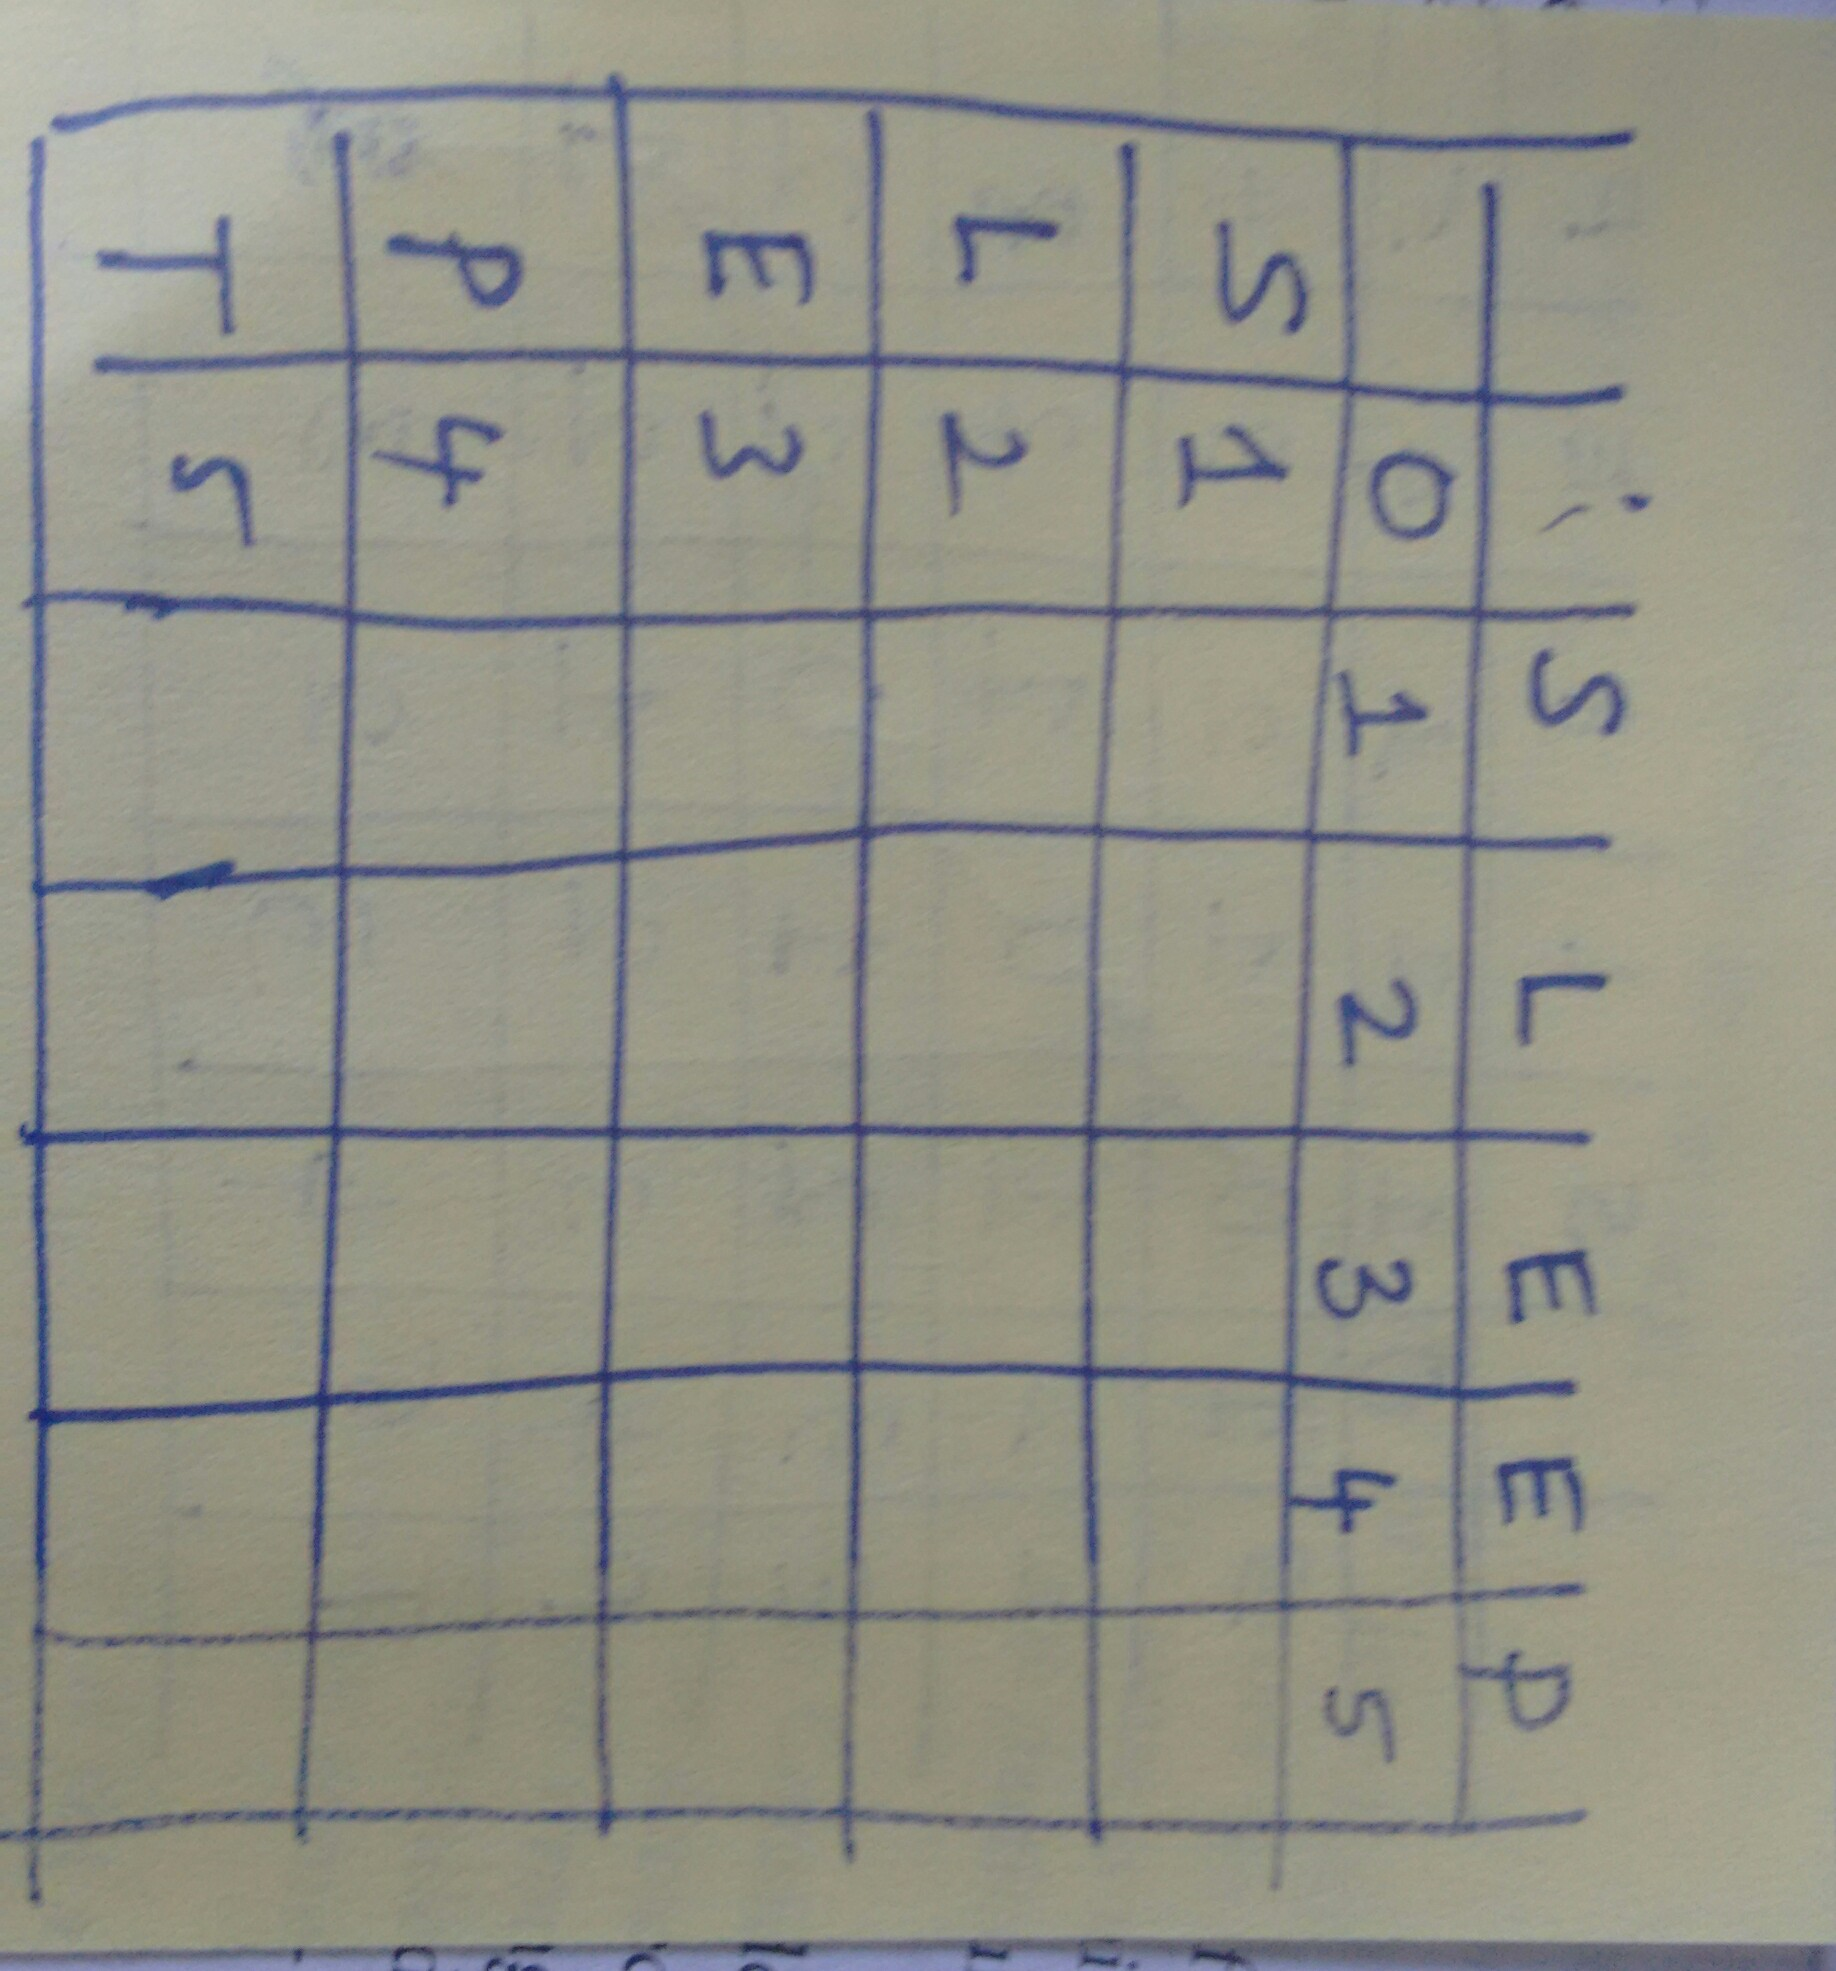
\includegraphics[width=0.6\textwidth,angle=90]{leven0.jpg}
\end{frame}

\begin{frame}
\frametitle{}
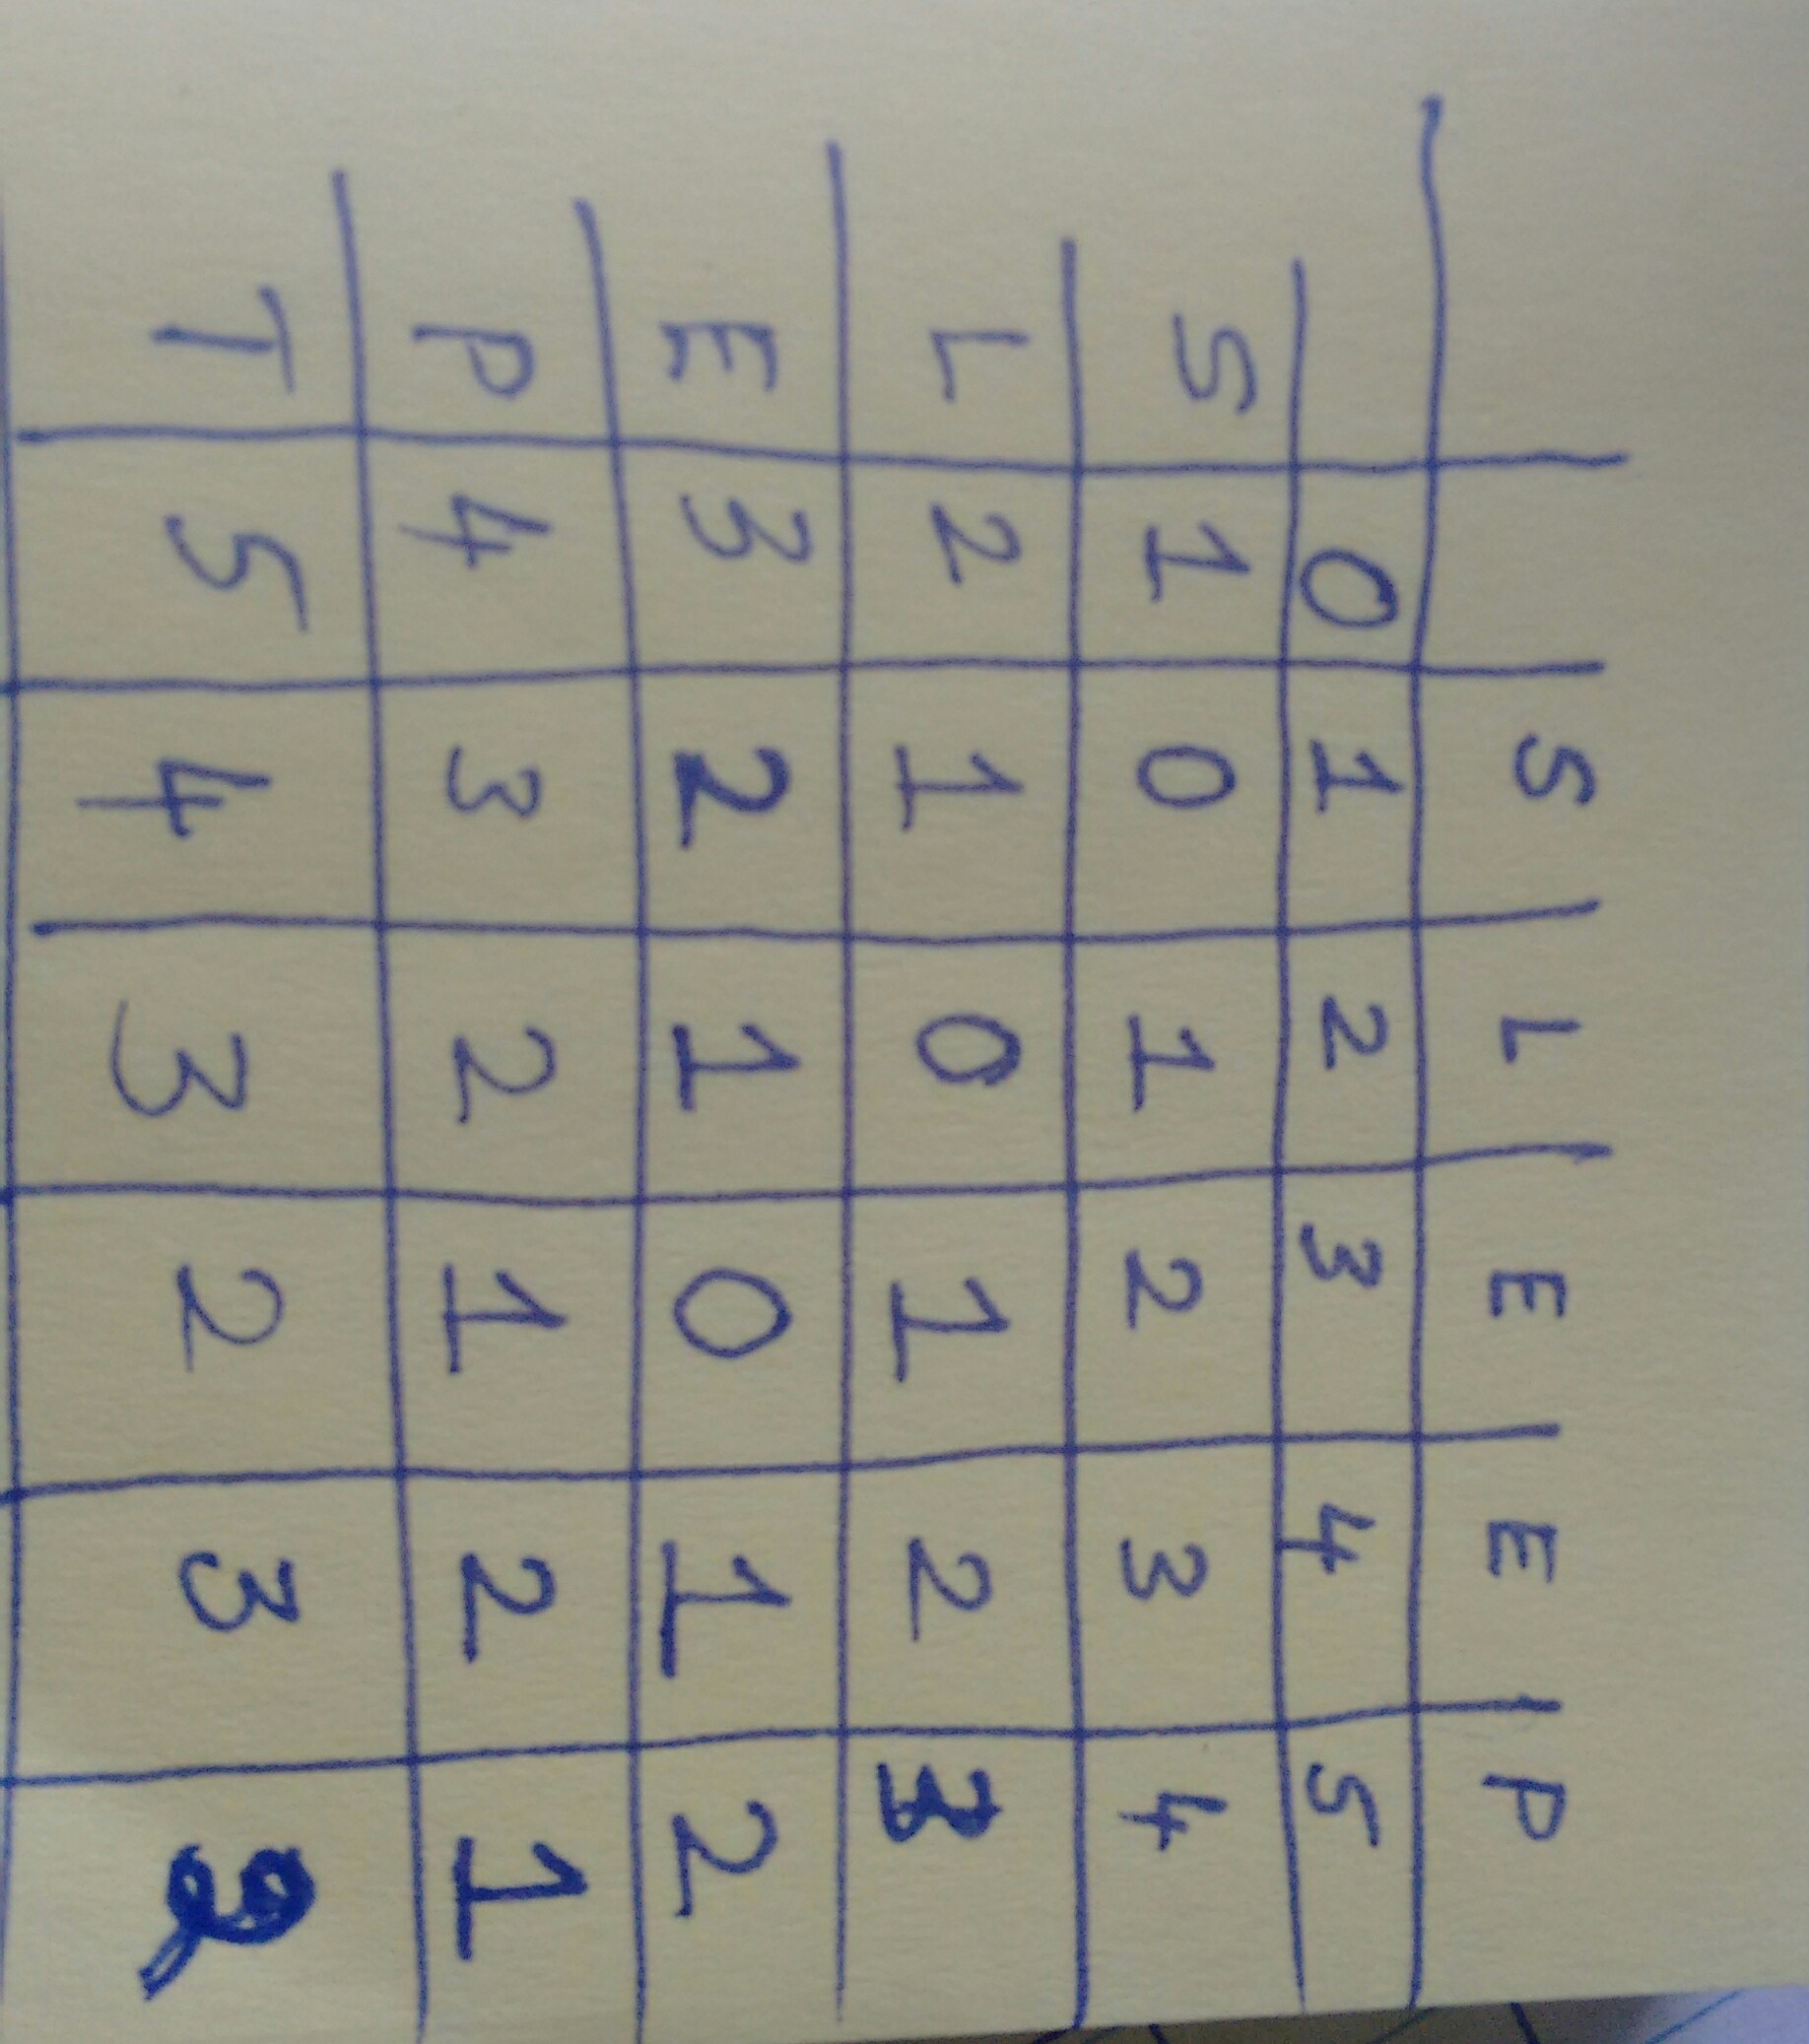
\includegraphics[width=0.6\textwidth,angle=90]{leven.jpg}
\end{frame}

\begin{frame}
\frametitle{}
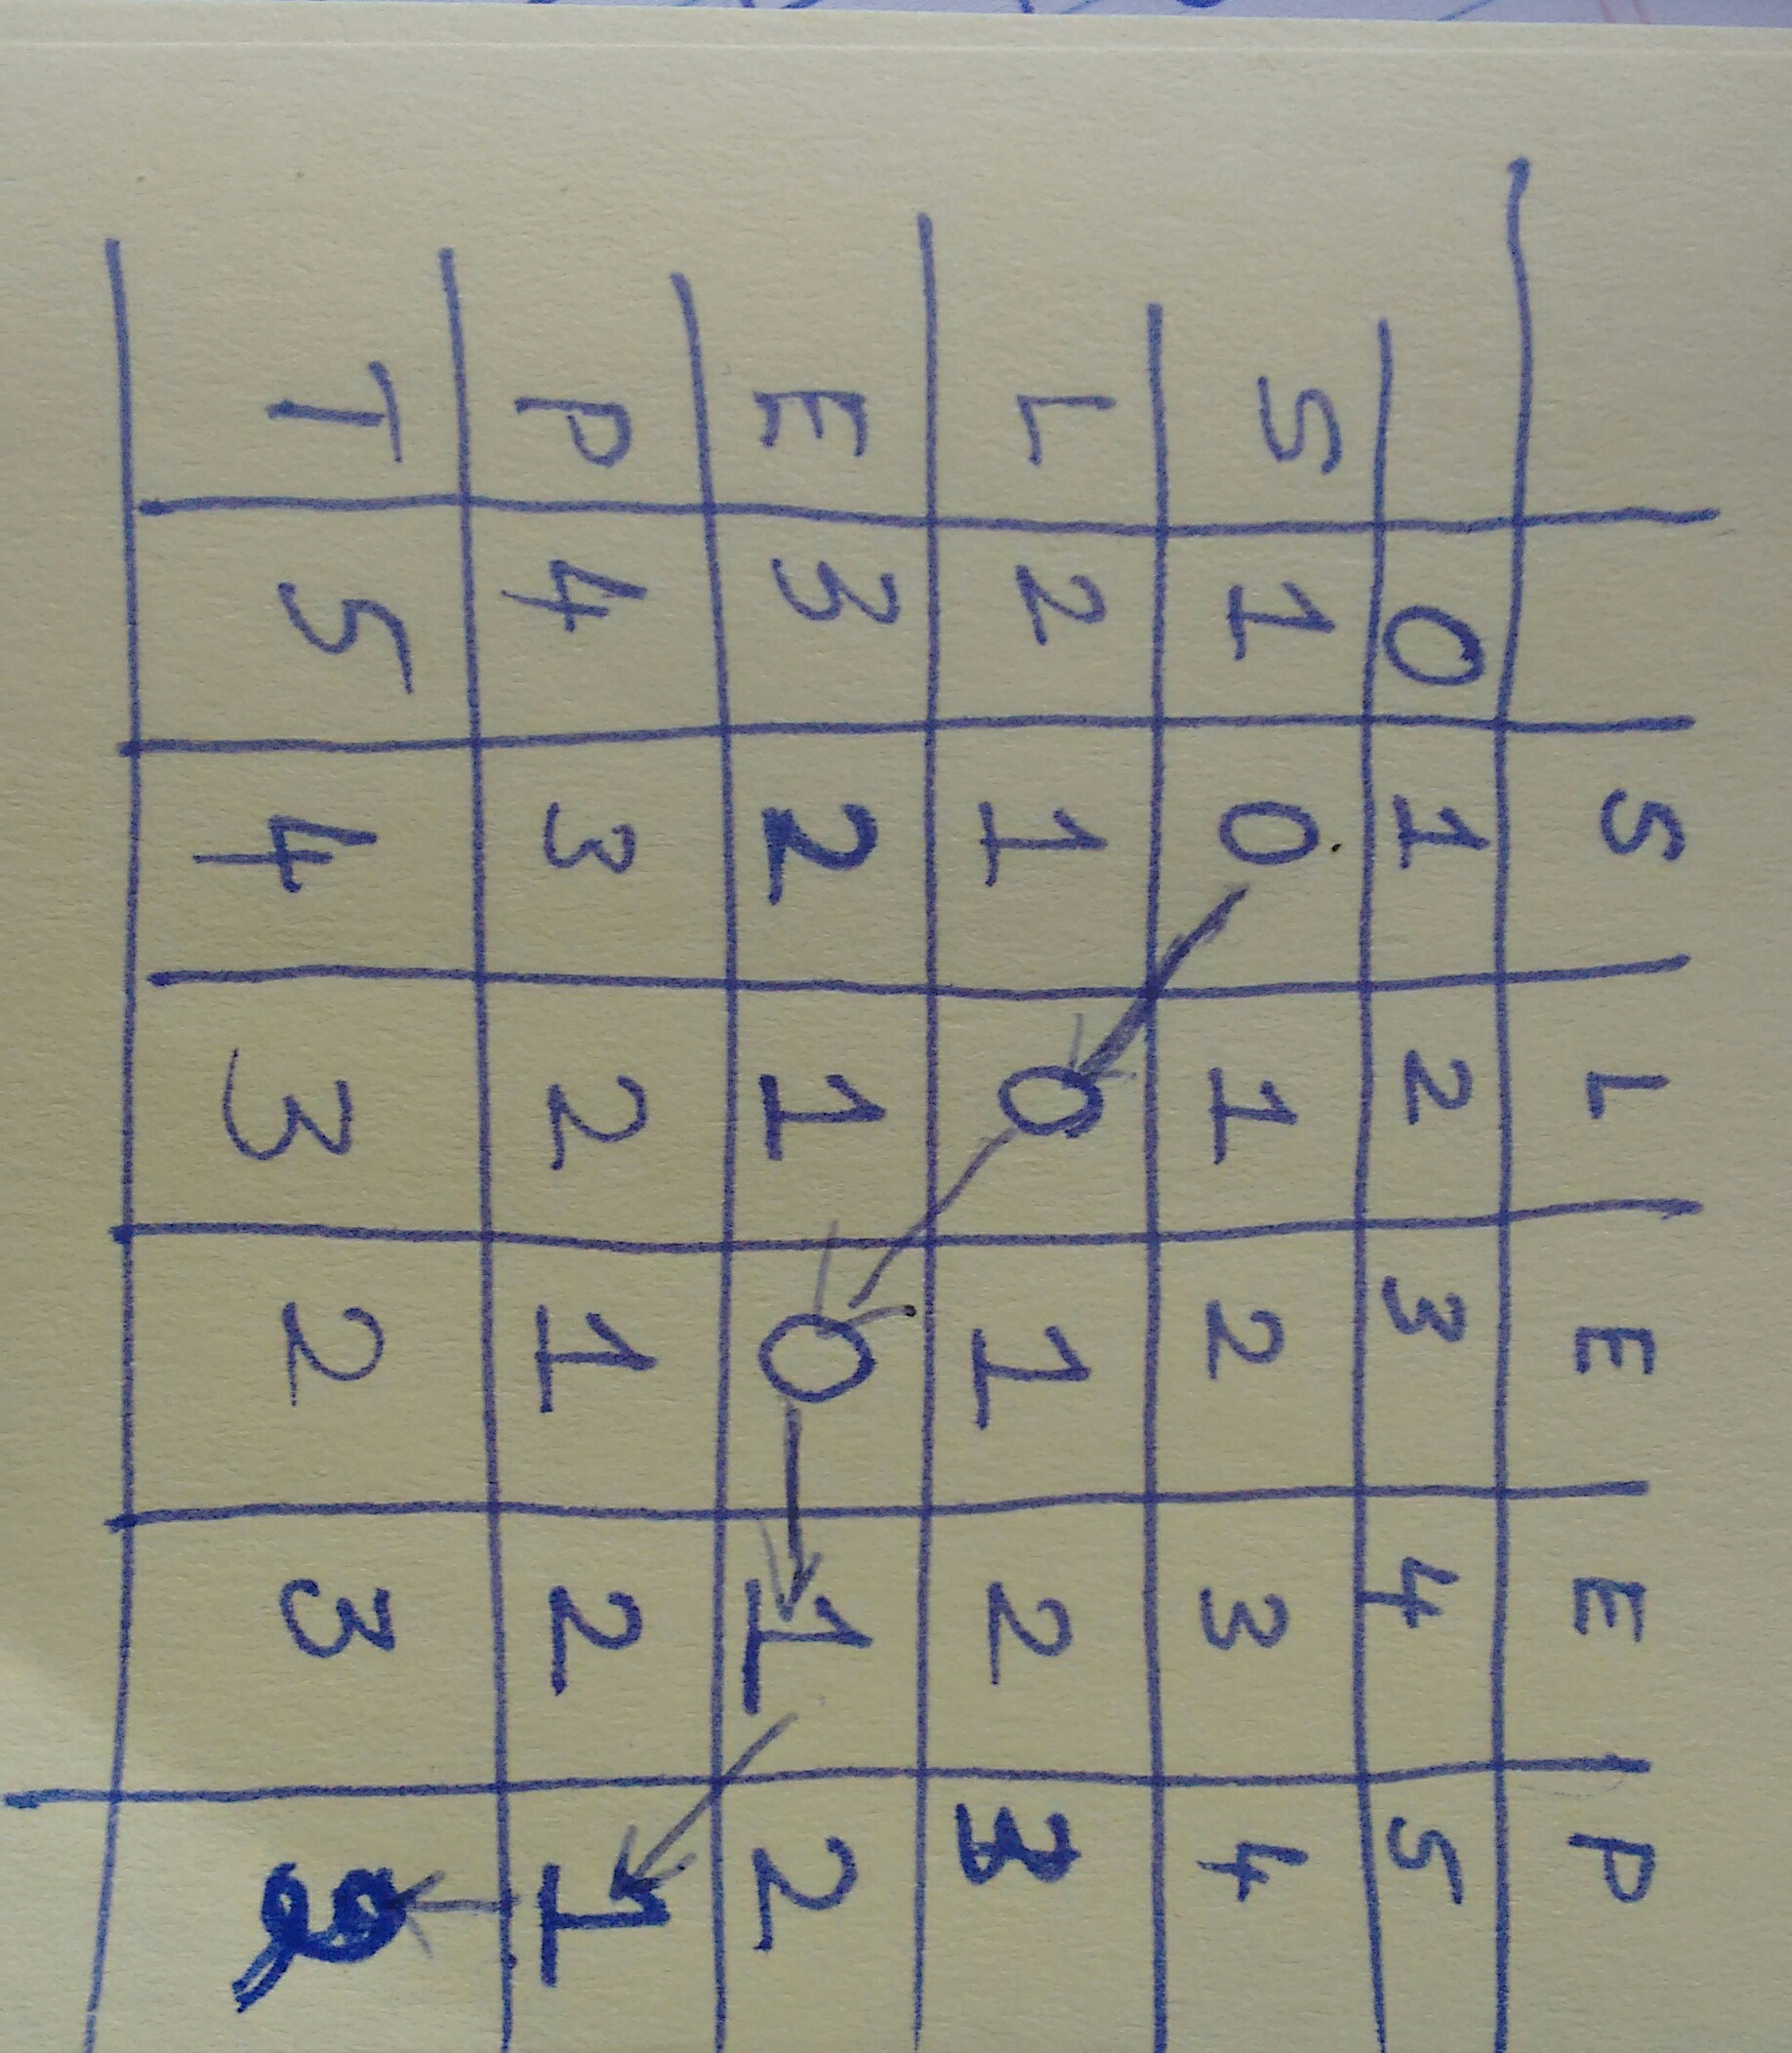
\includegraphics[width=0.6\textwidth,angle=90]{leven2.jpg}
\end{frame}

\begin{frame}
\frametitle{Pen and paper exercise}
Following the approach described just now, find the edit distance between google and goggles.
\end{frame}

\begin{frame}
\frametitle{Use for spelling correction/suggestions}
What you saw just now is an edit distance known as Levenshtein distance, and is used to suggest spelling alternatives, by choosing the closest words to the mis-spelt word. How we detect misspellings is for another day.
\end{frame}

\begin{frame}
\frametitle{Norvig's Spell Checker}
\begin{itemize}
\item How many people went back and had a look at Norvig's spell checker article and code? \pause
\item How many actually managed to run his code without getting errors (or how did you fix errors?) \pause
\item Did you make any changes to make it run interactively?
\end{itemize}
\end{frame}

\begin{frame}
\frametitle{Spelling suggestions in context}
\begin{itemize}
\item What does context sensitive spell checking mean? \pause
\item How do you think one can do context sensitive spell check? \pause
\item methods: ngram approaches, grammar checking rules etc. (More when we discuss NLP for CALL)
\end{itemize}
\end{frame}

\begin{frame}
\frametitle{Additional readings/lectures on this topic}
\begin{itemize}
\item Chapter on Writers Aids in Language and Computers by Dickinson et.al. 
\\ slides: \url{http://cl.indiana.edu/~md7/16/245/slides/02-writers-aids/slides.pdf}
\item Lecture 2.5 on edit distance in Radev's coursera course, Chapter 3.10-3.11 in J\&M. 
\end{itemize}
\end{frame}

\begin{frame}
\frametitle{Morphology for NLP: Quick Overview}
\begin{itemize}
\item Morphological analysis is an important component in speech and language processing. 
\item Plays an important role for web search (capturing all morphological variants of a word usage, for example)
\item Useful also in machine translation 
\item What is the big deal about morphological processing for NLP? If we have all word forms possible for all words, isn't it just a plain dictionary lookup?
%productive language, impossible t list all possibilities, morph. rich lang. - total difficult situation.
\end{itemize}
\end{frame}

\begin{frame}
\frametitle{Morphemes}
\begin{itemize}
\item Morphemes: minimal, meaning-bearing units of language.
\item Stem: main morpheme of the word
\item Affixes: morphemes that add additional meanings or information to stems.
\item cars is a word with two morphemes - car (stem) and -s (affix)
\item Affixes: prefixes, suffixes, infixes (middle of the word), circumfixes (start and end of the word). 
\item clitic: a morpheme that is syntactically a word, but used in a reduced form with another word.
\end{itemize}
\end{frame}

\begin{frame}
\frametitle{Combining Morphemes}
4 ways: inflection, derivation, compounding, cliticization
\begin{itemize}
\item inflection: combining a stem with a grammatical morpheme, usually resulting in a word with same POS class (tag-tagged; car-cars)
\item derivation: combining a stem with a grammatical morpheme, usually resulting in a word with different POS class (derive-derivation; computer-computerize)
\item compounding: combining multiple word stems (greenhouse, redhead)
\item cliticization: combining words with a clitic (we've, I'm)
\end{itemize}
\end{frame}

\begin{frame}
\frametitle{Additional Readings/Lectures on this topic}
\begin{itemize}
\item Survey of (mostly) English morphology (Chapter 3.1 in J\&M)
\item Lectures 2.01 to 2.04 in Radev's coursera course.
\item I will continue with this topic on tuesday, and talk about Stemming and Lemmatization
\end{itemize}
\end{frame}

\begin{frame}
\frametitle{Next Week}
\begin{itemize}
\item Topics: Morphological analysis - stemming and lemmatization, Introduction to n-gram approaches. 
\item Readings: Chapter 3--4 in J \&M, Chapter 5 in NLTK Book
\end{itemize}
\end{frame}

\begin{frame}
\frametitle{Practice exercises}
\begin{enumerate}
\item Figure out whether NLTK has a distance metric such as Levenshtein or other such orthographic distances, and learn how to use one such measure to get distance between words.
\item Check for any python based spell checking libraries. If you do not find any, learn to use PyEnchant library for spell checking. \pause
\item Start doing problems in Problem Set 2 (see Blackboard)
\end{enumerate}
\end{frame}

\end{document}


